\documentclass[journal]{IEEEtran}
\IEEEoverridecommandlockouts
\usepackage{cite}
\usepackage{amsmath,amssymb,amsfonts}
\usepackage{algorithmic}
\usepackage{graphicx}
\usepackage{textcomp}
\usepackage{xcolor}
\usepackage{graphicx}
\usepackage{epstopdf}
\usepackage{url}
\usepackage{bm}
\usepackage{bbm}
\usepackage{citesort}
\usepackage[super]{nth}
\usepackage{amsmath}
\usepackage{xcolor}
\usepackage{soul}
\usepackage{amsmath}
\usepackage{textcomp}
\usepackage{upquote}
\usepackage{cleveref}

\newcommand{\Hnull}{\mathcal{H}_0}
\newcommand{\Halt}{\mathcal{H}_1}
\newcommand{\Hb}{\mathcal{H}_b}
\newcommand{\Ones}{\mathbf{1}}
\newcommand{\Real}{\mathcal{R}}
\newcommand{\Imag}{\mathcal{I}}
\newcommand{\Hin}{{X}}
\newcommand{\Hout}{{Y}}
\newcommand{\Hini}{\mathcal{H}_i}
\newcommand{\Houtj}{\mathcal{D}_j}
\newcommand{\Honull}{\mathcal{{D}}_0}
\newcommand{\Hoalt}{\mathcal{{D}}_1}
\newtheorem{theorem}{\noindent \textit{Theorem}}
\newtheorem{lemma}{\noindent \textit{Lemma}}
\newtheorem{proposition}{\noindent \textbf{Proposition}}


\hyphenation{op-tical net-works semi-conduc-tor}


\begin{document}

\setstcolor{red}

\title{Location Verification for Emerging Wireless Vehicular Networks}

\author{

Ullah Ihsan, \IEEEmembership{Student Member, IEEE,} Shihao Yan, \IEEEmembership{Member, IEEE,} and Robert Malaney, \IEEEmembership{Senior Member, IEEE}

\thanks{U. Ihsan and R. Malaney are with the School of Electrical Engineering and Telecommunications, The University of New South Wales, Sydney, NSW 2052, Australia
(e-mails: \{ihsanullah, r. malaney\}@unsw.edu.au).}
\thanks{S. Yan is with the School of Engineering, Macquarie University, Sydney, NSW 2109, Australia. He is the corresponding author of this article (e-mail: shihao.yan@mq.edu.au).}
}

\markboth{Submitted to IEEE Internet of Things Journal}{Ihsan \MakeLowercase{\textit{et al.}}: Location Verification for Emerging Vehicular Networks}

\maketitle

\begin{abstract}

The work reported here utilises the best aspects of information theory and deep-learning concepts so as to provide, for the first time, a solution for a real-world Location Verification System (LVS) in the context of vehicular networks. It is well established that Global Positioning System (GPS) coordinates supplied by vehicles will be a vital component of such emerging networks. \textcolor{red}{\textit{This supplied location information, if erroneous and not verified, can seriously degrade the overall system performance and lead to significant safety issues. A number of location verification protocols and systems \cite{sheet2016location,kasana2017location,yan2014optimal,yan2016location,yan2016LOCATION,monteiro2016information} have been developed to address this important problem but all have operational constraints and performance limitations due to their requirement for ideal static channel conditions and assumed threat models.}} In this work we remove such limitations by designing a neural-network based LVS (NN-LVS) that can accommodate \emph{a priori} unknown channel conditions and unknown threat models.
\textcolor{red}{\textit{We also derive a new information-theoretic bound on the Total Error for an LVS and show how this new bound allows for a very useful trade-off in learning-time \emph{vs}. verification-performance. The work reported here, we believe, paves the way to the actual deployment in real-world condition of LVSs for emerging vehicular networks.}}

\end{abstract}

\begin{IEEEkeywords}
        ITS, VANET, Internet of Things, artificial intelligence, neural networks, location verification
\end{IEEEkeywords}

\section{Introduction}
Location information will play a pivotal role in many emerging networks - the Internet of Things, Trusted Autonomous Systems, and Vehicular Ad-hoc Networks (VANETS) being just a few. Indeed, it could be argued that location information on the physical entities that form such networks will form the most important knowledge attribute of the system. Because of this, the verification of such location information will play a crucial role in many aspects of network operations, with reliability and safety being of particular importance in the case of the emerging vehicular-network paradigm.
The notion of an Intelligent Transportation System (ITS) has been a research topic in the wireless telecommunication industry for well over a decade now. VANETS are a specific type of ITS that enables vehicle-to-vehicle and vehicle-to-infrastructure communications \cite{hartenstein2008tutorial}. %\cite{1}%\cite{hartenstein2008tutorial}
Amongst other goals, VANETS aim to minimise traffic congestion, provide for greener cities, improve road-tolling infrastructure, advertise nearby facilities, and allow for seamless integration of new
wireless entertainment services.  However, much-improved safety outcomes are arguably the most hoped-for consequence of deployed VANETS.  According to the World Health Organization, the number of fatalities World-wide due to traffic accidents were 1.25 million in 2013 \cite{who}. %\cite{2}
Elimination (or drastic reduction) of such a catastrophic death toll is a challenge that is yet to be fully addressed. It is a challenge that motivates all future vehicular-network deployments.

Location information forms the basis of almost all network decisions in VANETs. Within  most vehicular network architectures, a vehicle usually obtains its position from the Global Positioning System (GPS), perhaps with assistance from other components of the wider GNSS. The Wireless Access in Vehicular Environments (WAVE), specified in the IEEE 1609 family of standards \cite{meneguetteintelligent}, dictates that such location information is periodically reported to the wider network. A possibility exists whereby a malicious vehicle, in order to get an advantage over other vehicles, or to disrupt the system, or to trigger an unavoidable collision, can deceive the wider network by forging its location. Alternately, there is a possibility that a GPS receiver may wrongly calculate a vehicle's location due to poor reception or other non-malicious circumstances. Such events, if not carefully considered, can result in a host of undesirable outcomes.

Due to such considerations numerous algorithms for validating a vehicle's location in VANETS have been proposed over the past few years \cite{yan2013location}. These algorithms, in general, make use of a network infrastructure that comprises Road Side Units (RSUs) and vehicles. RSUs are static Base Stations (BSs) placed at optimum locations to assist VANETs with a range of communication objectives. The inter-vehicle, RSU-to-vehicle and vehicle-to-RSU communication data is processed by an RSU in a specified coverage area so at best facilitate network operations. However, in the context of location verification, these same signals can be utilized to verify all reported GPS positions.

\textcolor{red}{\textit{Researchers have formulated a number of information theoretic Location Verification Systems (LVSs) over the past few years \cite{yan2013location} which utilize available signal metrics, such as the Received Signal Strength (RSS) of a transmitted signal from a user-vehicle, the Time of Arrival (ToA) of the transmitted signal from the user-vehicle and/or the Angle of Arrival (AoA) of the transmitted signal from the user-vehicle, to validate the user-vehicle's reported location. At the same time these LVSs have certain operation limitations in terms of the channel conditions and can only work under the assumptions made at the time of their initial design. On the other hand, the use of artificial neural networks in an LVS provide a greater flexibility. Once trained to a certain limit, a neural-network based LVS (NN-LVS) can perform well in the environments they are designed for and also in conditions they are not intended for. As we will show the performance of an NN-LVS trained to a certain limit can be made comparable to one that has been trained for long time.}}

\textcolor{red}{\textit{The novel contributions in this work can be described thus.}}
\begin{itemize}
\item \textcolor{red}{\textit{We introduce for the first the time the concept of location verification within vehicular networks using neural network techniques.
\item The NN schemes we develop deploy new techniques based on optimal-decision-theory frameworks that significantly reduce the training phase with only a minimal impact on performance.
\item We study threat model under changing distance constraints for the malicious user in an environment that closely relates to the real-world conditions and show how our newly designed NN-LVS beats the performance of an information theoretic LVS.
\item We investigate in detail a specific example of these conceptual NN frameworks by determining a new theoretical lower bound on the optimal information-theoretic performance of location verification within the context of Non-line of site (NLoS) effects as described by an exponential distribution of bias.
\item By using this new lower bound we quantify the trade-off in NN training time \emph{vs.} performance, showing how traditional training times (using traditional stopping criteria) can be cut substantially while impacting on the total error only marginally.
\item We numerically investigate the performance of our new NN location verification systems under a wide range of generalised conditions in which the incoming data is substantially different from the test data used to train the NN.}}
\end{itemize}
In this work we first review LVS deployment issues. We then briefly review  techniques that have been proposed to address the location verification problem within VANETS; discussing a range of location verification techniques that are more of a  heuristic nature, before bringing our attention to  formal techniques based on optimal-decision theories. We then briefly introduce the use of Artificial Intelligence (AI) in the guise of neural-network architectures and  discuss their usefulness for location verification. \textcolor{red}{\textit{We then study the performance of our newly designed NN-LVS against a state-of-the-art information theoretic LVS when the threat model for the malicious user is randomly changing.}}We then derive new information-theoretic bounds on the performance of an LVS in the context of biased timings in realistic channel conditions before quantifying how the interplay between information theory and AI leads to improved location verification outcomes.

\section{Previous Works}

\subsection{Location Verification Deployment}
In a configuration of a vehicular network where a LVS is deployed, several of the vehicles will have been already authenticated, but vehicle 2, say, has not. Vehicle 2 sends a request to join the network and reports its GPS position through its nearest RSU to the LVS server. All RSUs and nearby vehicles hearing this request report any relevant signal metrics (e.g. signal strengths) back to the server.  The LVS server acts on this information, processing it to arrive at a verification decision. This decision is then reported back to all other vehicles in the network (or at least those in the vicinity of the requesting vehicle). In the case where the reported GPS position is not verified, the requesting vehicle has its security certificates revoked \cite{meneguetteintelligent}.
This communications system upon which this process is deployed over is quite generic and versatile. Dedicated Short Range Communications (DSRC), and the larger WAVE suite of protocols can easily accommodate the above configuration \cite{meneguetteintelligent}.
Vehicular network communications built on emerging 5G standards could also be easily accommodated.

\subsection{Heuristic Algorithms}
Most of the works prior to 2012 that have addressed the location verification issue within wireless networks have been extensively reviewed elsewhere \cite{yan2013location}. The most well-known of these early proposals are perhaps those of \cite{sastry2003secure,capkun2006secure,leinmuller2006position,harsch2007secure,rasmussen2008secure,yan2008providing}.

The `ECHO' protocol, based on the use of both radio and ultrasound frequencies, was developed in \cite{sastry2003secure}. The main advantage of this protocol is that it is largely independent of the tight synchronization (timing) requirements demanded by other schemes. In this protocol, the verifier sends a packet with an unknown random value to the claimant. The claimant then instantly responds, via ultrasound, upon receiving the packet. The verifier then compares the round-trip time against an ideal delay time. If the time-of-flight is less (more) than the ideal time, the claimant is marked to be inside (outside) the region.

A `verifiable multilateration' scheme was proposed in \cite{capkun2006secure}. The scheme is based on the notion of `distance bounding' (a malicious node can only claim he is further from the verifier not closer) and makes use of a minimum of three verifiers. The scheme can be shown to produce verifiable regions of space under a series of different threat models.

In \cite{leinmuller2006position}, a series of autonomous sensors were adopted which looked at a range of metrics, such as the anticipated range of communication, the anticipated maximum speed of vehicles, and the anticipated density of vehicles. Using techniques akin to malicious behavior detection in intrusion detection algorithms, a location verification outcome was derived.

A time stamp embedded within the packet that contains the claimed location was used to detect malicious vehicles in~\cite{harsch2007secure}. The time stamp check ensures that the received packet is neither in the appropriate time window.

In \cite{rasmussen2008secure}, the notion of covert BSs (BS whose locations are assumed to be unknown to the attacker) were introduced into the location verification problem. In conjunction with the use of secret keys, the use of covert BSs was shown to significantly improve the verification performance.

Finally, in \cite{yan2008providing} an onboard radar system was used to verify the vehicle's claimed location. Taking noise into account, the scheme detailed in \cite{yan2008providing} separately determines the GPS position tolerance shadow and radar position tolerance shadow - with the algorithm accepting (rejecting) the prover's claimed location if there is (is not) an intersection between the GPS and radar position shadows.

More recent works on the issue of location verification in VANETs have appeared post 2012 \cite{sheet2016location,kasana2017location,zhang2012cooperative,malandrino2013vip,jaballah2013secure,kim2017efficient,caparra2017optimization,vaas2018get}. In \cite{sheet2016location}, a tile-based system was used to construct aggregated `belief' type algorithms that include the use of nearby vehicles as a means to influence the belief value. \textcolor{red}{\textit{To reduce the impact of erroneous location information on future location prediction for an optimum geographical routing, the authors in \cite{kasana2017location} proposed a protocol named Location Error Resilient Geographical Routing (LER-GR). The protocol of \cite{kasana2017location} utilizes the errors in location information on nearby vehicles in choosing the next forwarding vehicle to further improve the geographical routing and overall network performance.}} In \cite{zhang2012cooperative}, the location verification problem was extended to a larger cooperative framework by using other vehicles. In \cite{malandrino2013vip}, the location of the vehicle was verified conditioned on a guarantee of privacy to the user. In \cite{jaballah2013secure}, the integration of location verification with a popular alert-message algorithm was investigated. The use of token-based registration models and the use of multiple (and independent) authentication rounds were
discussed in \cite{kim2017efficient}.  Power-optimization issues, in the context of location verification, were examined in \cite{caparra2017optimization}, while in \cite{vaas2018get} the use of vehicle trajectories in aiding the location verification was studied.

\subsection{Optimal-Decision Theory for Location Verification}
The major difference of an LVS compared to a positioning system is that an LVS provides a binary output (either a `True' or a `False' value) as an output decision regarding the location of a user, while a positioning system outputs an estimated position. The generic operational procedures of an LVS involve inputs that include the `claimed location' of a user along with independent signal inputs such as RSS, ToA, and/or AoA. After processing these inputs, the LVS labels the user's reported (claimed) position to be either true or false.
We note that an LVS solves a different problem than the determination of the location of a node in a secure fashion. In an LVS, we are focussed on authenticating the validity of a claimed location reported by a node, and not on a node self-locating itself in a secure manner.

We consider the following scenario for a general LVS. A claimed location for a vehicle (usually a GPS position reported by that vehicle) is provided as input to the LVS processor along with the channel metrics (e.g., RSS, ToA, or AoA). The assumed channel conditions between the verifier and claimant vehicles will form part of the integrated system model adopted by the LVS. In general, it is assumed that the verifier's locations are known and trustworthy. It could be that the verifiers are RSUs or other vehicles that have been previously authenticated. The LVS processor acts on these inputs with some pre-determined algorithm so as to produce a binary decision regarding the validity of the claimed location reported by the vehicle. A `true' means that the reported location is legitimate or trustworthy, while a `false' means that the reported location has not passed the verification test and the corresponding vehicle is likely spoofing its location (or its on board GPS is unreliable). This information can then be distributed to the wider network and it can be left up to individual vehicles, or the network system as a whole, on how to act on that information. In most situations a vehicle failing the location verification test will have its security certificates revoked \cite{meneguetteintelligent}. The nature of the specific algorithm deployed within the LVS can be wide and varied, ranging from simple heuristic algorithms to those using optimal information-theoretic techniques, which will be discussed in the following.

Several location verification frameworks for VANETs, using optimal-decision theories, were formulated in a series of papers~\cite{yan2014optimal,yan2016location,yan2016LOCATION,monteiro2016information}. In the first of these works, the mutual information between the input and output LVS data was used as the objective optimization criterion. It was proven how a likelihood ratio test, constructed from the probability of receiving a specific RSS value under different binary hypothesis (the claimant is truthful or untruthful), leads to an optimal decision~\cite{yan2014optimal}.  The work was extended in \cite{yan2016location} to correlated-shadowing environments where a more general optimization criterion based on the Total Error  was utilized. The Total Error is a combination of the fraction of false positives (friendly vehicle stating a true location marked as malicious) and the fraction of missed detections (malicious user spoofing a location marked as friendly). The use of optimal decision theory based on Total Error in the context of Rician channels (the most likely form of channel in many vehicular environments) was reported in \cite{yan2016LOCATION}. In \cite{monteiro2016information}, the use of directional antennas within the context of optimal decision theory and location verification for vehicular networks was reported, showing how the use of such antennas can increase verification performance.

\subsection{Inclusion of Artificial Intelligence}
The LVS processing discussed above will provide for the optimal decision conditioned on one important assumption - that the wider system model adopted is reality. However, in practice the adopted system model can only be considered an approximation to reality. This is because inferred channel conditions, noise parameters, receiver characteristics, position-error assumptions, and other system descriptors are very difficult to \emph{a priori} determine. The issue is further complicated by the fact that the system parameters are likely to possess both spatial and temporal characteristics. To accommodate such real-world issues, a more sophisticated solution beyond optimal-decision frameworks will be desired. This additional ingredient, we believe, will be Artificial Intelligence (AI) or machine learning.

AI  within the context of vehicular networks has been discussed previously. It is considered that AI will play an important role in many characteristics of the vehicular networks, all the way through from vehicle classification problems, vehicle vision systems, autonomous driving, big-data analytics, routing, vehicle security, and driver behaviour, to name just a few (see \cite{fridman2017autonomous} and references therein for an overview).

It is part of our own ongoing work in this area to seamlessly integrate optimal decision LVS frameworks within AI architecture for location verification. We believe the combination of these techniques will provide for a `best of both worlds' approaches to this important problem. The optimal decision theory will be used as part of the initial training set for the machine learning, and will be utilised in circumstances when the AI algorithm has not been trained for the specific locale being investigated.  Once trained under ideal conditions, the deep-learning algorithms within the architecture will then be adjusted under real-world conditions when enough authenticated vehicles can be utilised as part of the training set.

\section{The System Model}\label{system_model}

\subsection{The New LVS}
A schematic of our combined AI architecture is given in Fig.~\ref{Figure3}.
\begin{figure}[t!]
\centering
\includegraphics[width=0.5\textwidth]{Figure3.eps}
\caption{Inclusion of Artificial Intelligence into the LVS.\label{Figure3}}
\end{figure}
Here we see how the optimal decision theory outputs can be used as part of the initial training phase, as well as the ongoing training phase (as more vehicles are authenticated or marked malicious). The mutual information between the outputs of the optimal-decision theory and the AI can be used as an additional input to the AI deep-learning algorithms, as well as providing a measure of `agreement' between the two processes. Confidence levels associated with this measure could further assist the LVS.
\subsection{Adopted System Model Assumptions}
Building on the work of \cite{Ausctw} we assume the following.

\begin{enumerate}

\item {A \emph{single} vehicle to be identified (henceforth referred to as the user-vehicle) reports its claimed location, $\bm{\theta}_c = [x_c,y_c]$, to a network with $N$ verifiers. Verifiers are fixed BSs with known locations. The location of the $i$-th BS is $\bm{\theta}_i = [x_{i},y_{i}]$ ($i = 1, 2, \dots, N$). We select one of the $N$ BSs as the Process Center (PC) - which collects all measurements.}

\item {A vehicle (legitimate or malicious)  obtains its true position, $\bm{\theta}_t = [x_t,y_t]$, from  GPS with zero localization error. A legitimate vehicle's claimed (reported) position, $\bm{\theta}_c$, is taken to be identical to its true position $\bm{\theta}_t$. A malicious vehicle will falsify (spoof) its claimed position in an attempt to fool the LVS. The malicious vehicle's true location is unknown and its (spoofed) claimed  location is  taken to be $\bm{\theta}_c$.}

\item {We denote the null hypothesis where the user-vehicle is legitimate as $\Hnull$, and denote the alternative hypothesis where the user-vehicle is malicious as $\Halt$. This can be summarized as,
\begin{eqnarray}\label{prior}
 \left\{ \begin{aligned}\label{ncon}
        \ & \Hnull:~\bm{\theta_c} = \bm{\theta_t}\\
        \ & \Halt:~\bm{\theta_c} \neq \bm{\theta_t}.
         \end{aligned} \right.
\end{eqnarray}}
\end{enumerate}

\subsection{Observation Model under $\Hnull$}

The ToA measured at the $i$-th BS from a legitimate vehicle, $Y_i$, is given by
\begin{eqnarray}\label{observ_H0}
Y_i = U_i + X_i + \phi_i, ~~i = 1, 2, \dots, N,
\end{eqnarray}
where
\begin{eqnarray}\label{equation_9}
U_i = \frac{d_i^c}{c},
\end{eqnarray}
and $d_i^c$ is the Euclidean distance of the $i$-th BS to a user-vehicles's true location (also its claimed location) given by $d_i^c = \sqrt{(x_c - x_i)^2 + (y_c - y_i)^2}$, $c$ is the speed of light, $X_i$ is a zero-mean normal random variable with variance $\sigma_{T}^2$, which represents the additive noise term in the ToA measurements, and $\phi_i$ is a random variable (in ns) that represents the bias caused by non-line-of-sight (NLoS) channel conditions, that follows an exponential distribution with $\rho_i$ as the scale parameter, i.e.,
\begin{align}\label{exponential_bias}
f(\phi_i) = \rho_i e^{-\rho_i \phi_i}.
\end{align}
 In the first instance we adopt the exponential distribution to model the bias term in the ToA measurements, since this bias  should be always positive due to the NLoS channel conditions.

We assume that the observations collected by different BSs are independent and thus the likelihood function of the $N$-dimensional observation vector under $\Hnull$ is given by
\begin{equation}\label{likelihood_H0}
f\left(\mathbf{Y}|\Hnull\right) = \prod_{i=1}^N f\left(Y_i|\Hnull\right),
\end{equation}
where $f\left(Y_i|\Hnull\right)$ is the likelihood function of each $Y_i$ under $\Hnull$. We will derive the explicit expression of $f\left(Y_i|\Hnull\right)$ later to facilitate the determination of the likelihood function $f\left(\mathbf{Y}|\Hnull\right)$.

\subsection{Observation Model under $\Halt$}

It is reasonable to assume that the malicious vehicle's true location is not close to its claimed location when an attack occurs.   Note also,  the malicious vehicle can alter some system parameters to interfere  with the observations collected by all BSs. As such, the ToA measured at the $i$-th BS, $Y_i$, is given by
\begin{eqnarray}\label{observ_H1}
Y_i = T_x + W_i + X_i + \phi_i, ~~i = 1, 2, \dots, N,
\end{eqnarray}
where
\begin{eqnarray}
W_i = \frac{d_i^t}{c},
\end{eqnarray}
and $T_x$ is the time bias utilised by the malicious vehicle, and $d_i^t$ is the Euclidean distance of the $i$-th BS to a user-vehicle's true location given by $d_i^t = \sqrt{(x_t - x_i)^2 + (y_t - y_i)^2}$. Since all BSs can communicate with each other,  $T_x$ is a constant value as seen by all BSs. Again, assuming that the observations collected from different BSs are independent, the likelihood function of the $N$-dimensional observation vector $\mathbf{Y}$ under $\Halt$ is given by
\begin{equation}\label{likelihood_H1}
f\left(\mathbf{Y}|\Halt\right) = \prod_{i=1}^N f\left(Y_i|\Halt\right),
\end{equation}
where $f\left(Y_i|\Halt\right)$ is the likelihood function of each $Y_i$ under $\Halt$. In general, the malicious vehicle will optimally set the value of $T_x$ in some sense in order to minimize the probability to be detected. We denote the optimal value of $T_x$ as $T_x^{\ast}$.
We will assume in the calculations to follow that the malicious vehicle optimizes $T_x$ through minimizing the KL-divergence between $p(\mathbf{Y}|\Hnull)$ and $p(\mathbf{Y}|\Halt)$, where $p(\mathbf{Y}|\Hnull)$ and $p(\mathbf{Y}|\Halt)$ are the likelihood functions of observations under $\Hnull$ and $\Halt$, respectively This KL-divergence is defined as
\begin{equation}\label{KLdistance}
\begin{split}
D_{01}(p(\mathbf{Y}|\Hnull)|| p(\mathbf{Y}|\Halt)) &= \int p(\mathbf{Y}|\Hnull) \ln {\frac{p(\mathbf{Y}|\Hnull)}{p(\mathbf{Y}|\Halt)}} d{\mathbf{Y}}\\
&= \sum_{i=1}^{K} \frac{\left(U_i - W_i - T_x \right)^2}{2\sigma_{T}^2}.
\end{split}
\end{equation}
Then, the optimal value of $T_x$ can be obtained through
\begin{equation}\label{optimal Px}
\begin{split}
T_x^{\ast} &= \arg\underset{P_x}{\min}\,{D_{KL}\left(p(\bm{m}|\Hnull|| p(\bm{m}|\textcolor{red}{\theta_t}, \Halt)\right)}\\
&= \frac{1}{N}\sum_{i=1}^{N} \left(U_i - W_i\right),
\end{split}
\end{equation}
\textcolor{red}{\textit{where $\bm{m}$ is the mean measurement vector for ToA of the signal under the relevant hypothesis.}} The value of $T_x$ adopted by the malicious vehicle is not known to an LVS, and therefore the examination based on $T_x^{\ast}$ is applicable to the worst scenario for an LVS (best scenario for the malicious vehicle).

\subsection{Likelihood Functions and Performance Limits}

In this section, we first formalize the decision rule embedded in a ToA-based LVS. In order to  analyze the performance of this LVS, we also derive the likelihood functions, based on which we then discuss the strategy of the malicious vehicle to optimally set $T_x$. Finally, the performance limit of the LVS is examined.

\subsection{Binary Decision Rule}

In a localization system, the output is normally the estimated location of a vehicle. This is quite different from an LVS where the
 output is usually a binary yes/no decision. In this work we adopt the likelihood ratio test as the decision rule embedded in our LVS.  It has previously been proved that the likelihood ratio test can achieve the minimum Total Error, which is the sum of the false positive rate and detection rate (we will always assume in this work that the  \emph{a priori} probability of a vehicle acting maliciously is $P_0=0.5$\footnote{\textcolor{red}{\textit{The probability of a malicious attack is in fact an unknown input to an LVS. However, our own preliminary  study of  NN-LVSs dedicated to the impact of this unknown probability has shown that, in fact, it has very little impact on any NN-LVS \cite{Ihsan_ICC}.}}})\cite{neyman1933problem}. The decision rule based on the likelihood ratio is
\begin{equation}\label{arbitrary}
\Lambda\left(\mathbf{Y}\right) \triangleq \frac{f\left(\mathbf{Y}|\Halt\right)}{f\left(\mathbf{Y}|\Hnull\right)} \begin{array}{c}
\overset{\Hoalt}{\geq} \\
\underset{\Honull}{<}
\end{array}%
1,
\end{equation}
where $\Lambda\left(\mathbf{Y}\right)$ is the likelihood ratio, and $\Honull$ and $\Hoalt$ are the binary decisions that infer whether the prover is legitimate or malicious, respectively. Given the decision rule in \eqref{arbitrary}, the false positive rate and detection rate of an LVS are mathematically given by $\alpha = \Pr(\Hoalt|\Hnull)$ and $\beta = \Pr(\Hoalt|\Halt)$, respectively. Then, the Total Error is given by,
\begin{equation}\label{TE_old}
\xi = 0.5(\alpha + 1 - \beta).
\end{equation}
We note that the decision rule given in \eqref{arbitrary} can achieve the minimum value of $\xi$, which is denoted by $\xi^{\ast}$.

\section{Numerical Results on LVS}\label{numerical_results_1}

\subsection{NN-LVS System Architecture}
\indent \textcolor{red}{\textit{Based on a series of trials with changing architectures for the NN-LVS, we have designed a NN-LVS that has an input layer, a hidden layer with 10 neurons, and an output layer with a binary output (true or false) that decides on the integrity of a user-vehicle's reported location. This neural network architecture provides better accuracy and robustness. The inputs to the NN-LVS are the same as those considered for the information theoretic LVS i.e. ToA of the transmitted signal and the claimed location from a user-vehicle.}}

\textcolor{red}{\textit{The activation function for a neuron in the hidden layer is given by,}}
\begin{eqnarray*}\label{NN_equation_1}
    a_{(h,n)}= b + w_{(h-1,1)}a_{(h-1,1)}+\dots+w_{(h-1,j)}a_{(h-1,j)},\\
    n,j=1,2,\dots ,N,\
\end{eqnarray*}
\textcolor{red}{\textit{where $b$ is a constant, $a$ is the activation for a neuron in a layer ranging from $1$ to $n$, $h$ represents the hidden layer and $w$ is the weight connecting a neuron in the input layer to the neuron in the hidden layer.}}

\textcolor{red}{\textit{Based on numerous rounds of simulation with changing transfer functions and backpropagation algorithms for the NN-LVS, we decided to utilize the hyperbolic tangent sigmoid transfer function in the hidden layer and the Levenberg Marquardt as the backpropagation algorithm.}}

\textcolor{red}{\textit{We supply the NN-LVS with training data\footnote{By training data we mean ToA data received from user-vehicles who we know \emph{a priori} to be legitimate or malicious. Use of such data in order to set the neural network parameters, prior to its use on `unlabeled' data (i.e., data from user-vehicles who we do not know \emph{a priori } to be legitimate or malicious), is known as the training phase. Knowing when to end this training phase is one of the key questions we answer in this work.} at a speed of one random user-vehicle ToA data per second. Once the ToA data is supplied, the NN-LVS (via the backpropagation algorithm) optimises its weights and biases through a process called $learning$. The most frequent condition that terminates the learning process is the backpropagation algorithm's gradient descent. The gradient descent refers to minimizing the cost function for the  NN-LVS through optimization of the weights as given below,}}
\begin{eqnarray*}
    w_i \leftarrow w_i-\alpha \frac{\partial}{\partial w_i}J(w_0,w_1\dots w_j),~~ i=1 \dots j,
\end{eqnarray*}
\textcolor{red}{\textit{where $\alpha$ (a dimensionless constant) is the learning rate and $J$ is the cost function for the NN-LVS. `$J$' is the mean square difference between the calculated output for the training data, and the ground truth available with the training data.}}
\begin{eqnarray*}
   J(w_0,w_1\dots w_j) = \frac{1}{2m}\sum_{i=1}^{m} (\hat{y} - y)^2,
\end{eqnarray*}
\textcolor{red}{\textit{where $m$ is the number of training examples in the training data, $\hat{y}$ is the calculated output for the training data, and $y$ is the ground truth available with the training data. The learning is terminated when $J_k \geq J_{k-1}$ over a set number of multiple iterations in a row (In our case this value is set to 6). `$k$' refers to the iteration number. Once the learning has concluded, the weights and biases for the NN-LVS are considered as tuned. The NN-LVS thereafter can be applied to the test data\footnote{The test data is simulated under a different realization with same settings as training data. Further, test data has no labels} to calculate binary outputs for classifying the user-vehicles.}}

\subsection{Effects of Bias and Assumed Threat Model}

\textcolor{red}{\textit{We now compare the NN-LVS's performance with the performance of the information theoretic framework formulated in \cite{Ausctw}. Our modelling of the channel for the malicious user-vehicle attempts to take into account the uncertainty implicit in any real-world channel for a malicious user-vehicle a distance $r$ from a claimed location. In reality, the  BS-vehicle channel for any user-vehicle (a malicious or otherwise) is complex, dynamic (principally due to vehicle motions) and unknown. No accurate  analytical theoretical model exists for such a real-world scenario. However, the key advantage of a NN-LVS over any purely information-theoretic LVS, is that the former can always `learn' the channel models for both the legitimate and the malicious user-vehicles. This is true for all real-world channels irrespective of their nature (other than a purely random channel).}}

\textcolor{red}{\textit{To make progress, and to test our NN-LVS numerically, we will model a specific real-world channel (roughly considered as a stochastic combination of bias and Rayleigh fading) for the malicious user-vehicle as follows. It is implemented in the following manner. Each measurement by the BS is probabilistically determined as either a pure bias term or a  pure scattering term (i.e. no LoS component) with the weighting of each term exponentially weighted with the distance $r$ through $e^{-ar}$ where $a$ is set to $\frac{1}{x}$, $x$ being the distance we expect the malicious channel to be  pure bias with probability $1/e$. Random Gaussian  noise is then added to the measurement. This channel model mimics the fact that as the malicious user-vehicle approaches the claimed location its channel model should approach that of a legitimate vehicle, and as it moves further from the claimed location the model  provides for equal timing measurements, moduli noise. The legitimate user-vehicle channel is always modelled as a pure bias channel. As we will see in our results the NN-LVS does indeed learn these `real-world channels' - an outcome that persists independent of the details of the  actual malicious/legitimate channel model adopted.}}

\textcolor{red}{\textit{The decision rule for the ToA based information theoretic LVS in \cite{Ausctw} is given by,}}
\begin{align} \label{LRT20}
\Lambda \left(\boldsymbol{Y}\right)=\frac{e^{\mathrm{-}\frac{1}{2}{\left(\boldsymbol{Y}-\boldsymbol{V}\right)}^{\mathrm{T}}\boldsymbol{\ }{\boldsymbol{R}}^{-1}\boldsymbol{\ }\left(\boldsymbol{Y}\boldsymbol{-}\boldsymbol{V}\right)}}{e^{\mathrm{-}\frac{1}{2}{\left(\boldsymbol{Y}-\boldsymbol{U}\right)}^{\mathrm{T}}\boldsymbol{\ }{\boldsymbol{R}}^{-1}\boldsymbol{\ }\left(\boldsymbol{Y}\boldsymbol{-}\boldsymbol{U}\right)}}\ \ \ \genfrac{}{}{0pt}{}{\genfrac{}{}{0pt}{}{\Hoalt}{\ge }}{\genfrac{}{}{0pt}{}{<}{\Honull}}\ \ \ \lambda,
\end{align}
\textcolor{red}{\textit{where $\Lambda \left(\boldsymbol{Y}\right)$ is the likelihood ratio, $\Hoalt$ and $\Honull$ are the binary decision values indicating whether the user is legitimate or malicious and $\lambda$ is the decision threshold.}}

\textcolor{red}{\textit{In our comparison study shown in Fig.~\ref{New_30}, we have four BSs in a 1000m X 500m area, and $X_i$ and NLoS bias have a fixed standard deviation of 100ns, and 300ns respectively. The LRT in equation \eqref{LRT20} gives a Total Error of 0.14 for $r$ = 150m, 0.10 for $r$ = 200m, 0.07 for $r$ = 300m, 0.06 for $r$ = 1000m and 0.07 for $r$ = 10000m. In comparison, the NN-LVS has a Total Error of 0.19, 0.14, 0.10, 0.04 and 0.01 for $r$ equal to 150m, 200m, 300m, 1000m, and 10000m respectively. Our comparison study shows that contrary to the information theoretic LVS of \cite{Ausctw}, the NN-LVS performs better and its Total Error improves with increasing $r$. This supports our claim that NN-LVS is good at learning channel conditions, has a steady performance, and is more dependable in real-world situations.}}
\begin{figure}[t!]
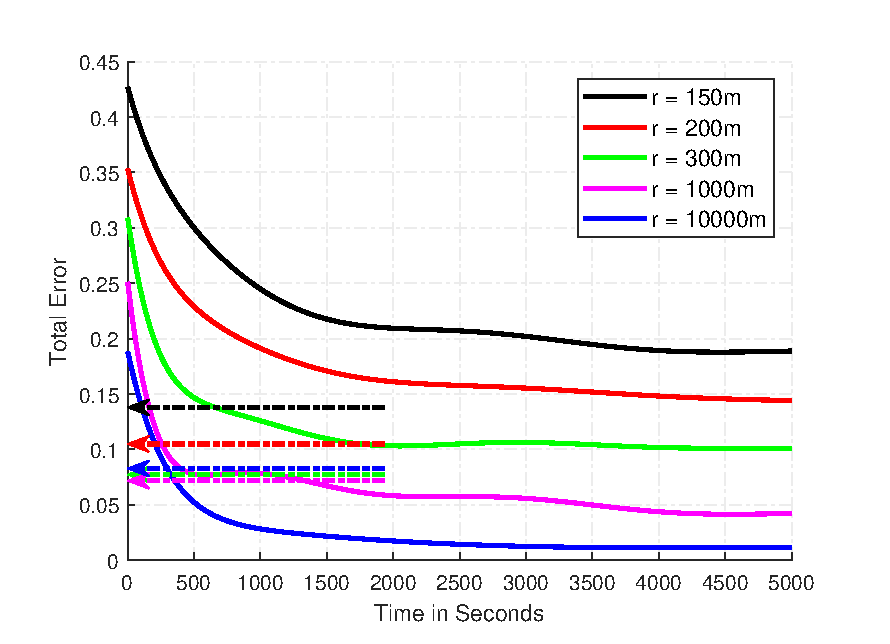
\includegraphics[width=0.50\textwidth]{final-T100-N300-V4-arrow.eps}
\caption{\textcolor{red}{\textit{Total Error performance for NN-LVS with four BSs and changing values of $r$. The scenario presented here closely relates to the real-world conditions where $X_i$ is extracted from a random Gaussian distribution and the NLoS bias is extracted from a random exponential distribution. $X_i$ and the NLoS bias have a fixed standard deviation of 100ns and 300ns respectively. The solid lines shows the Total Error performance for the NN-LVS under different values of $r$ while the dashed arrow lines point to the respective Total Error calculated on the basis of the LRT method presented in \cite{Ausctw}. The NN-LVS reports a continuous improvement in its performance with an increasing $r$.}}\label{New_30}}
\end{figure}

\textcolor{red}{\textit{We repeat the above comparison study in Fig.~\ref{New_31} by modifying the standard deviations for $X_i$ and NLoS bias to 300ns, and 100ns, respectively. All the other simulation parameters are the same as in Fig.~\ref{New_30}. We can see again that compared to the information theoretic LVS, the NN-LVS has a better performance.}}
\begin{figure}[t!]
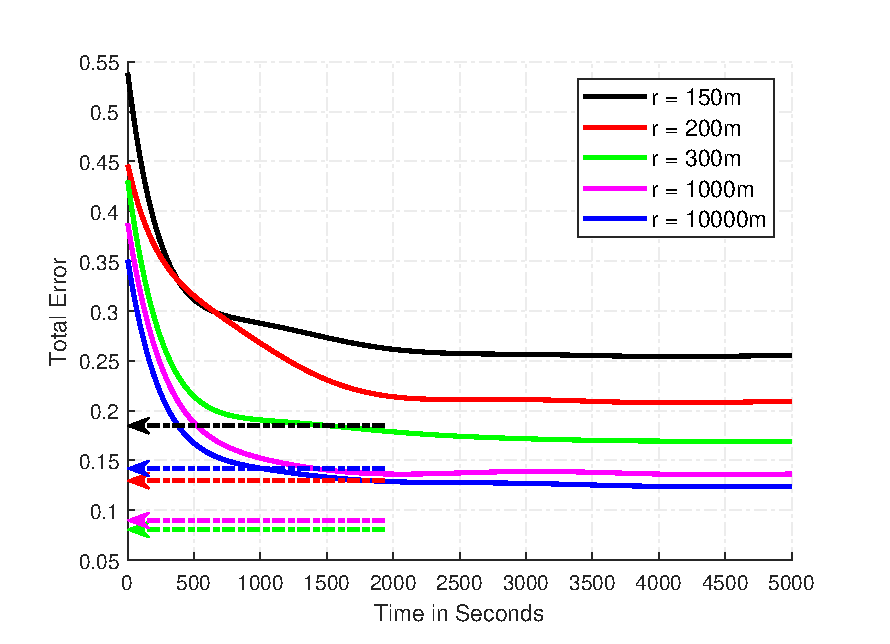
\includegraphics[width=0.50\textwidth]{final-T300-N100-V4-arrow.eps}
\caption{\textcolor{red}{\textit{Total Error performance for the NN-LVS as in Fig.~\ref{New_30} except the standard deviations for $X_i$ and NLoS bias have been modified to 300ns and 100ns respectively.}}\label{New_31}}
\end{figure}

\subsection{Other Network Issues}
\textcolor{red}{\textit{We note our calculations in this work assume that network congestion issues do not play a role. That is, we assume the messages containing all the information required for the LVS-based neural network calculations can be received  (and processed) in a timely manner. If the number of vehicles becomes too large such that communications with the nearby BSs are interfered with then clearly location verification processes will be curtailed. However, eventually we believe an LVS will be embedded directly within the WAVE architecture as described by the IEEE 1609 suite of standards and the IEEE 8011.p standard (see \cite{meneguetteintelligent} for discussion of all these standards). WAVE mandates the position information of all vehicles is broadcast every 100ms as part of the wider vehicular network safety messages, and moreover, that priority is given to these messages. The bandwidth available to such high priority messages within WAVE is designed so as to accommodate all anticipated network conditions. In this work we assume all LVS messages are treated the same as the position information messages.}}

%********************************************************************************
\section{A Theoretical Lower Bound on Total Error}\label{section_5}
\textcolor{red}{\textit{A quicker NN-LVS training stopping condition could be useful in that it can  save  training time,  training data costs, and make for a faster NN-LVS. To achieve this we introduce a new bound, referred to as the Total Error Lower Bound (TLB). This bound, as we will show, in conjunction with the usual learning process can  indeed result in a stopping of the NN-LVS training at an earlier time -  a time when the NN-LVS is performing adequately. The TLB is calculated using information theoretic analysis as we now discuss  assuming a priori knowledge on the distribution of the bias term at each BS.}}

\subsection{Likelihood Functions under $\Hnull$ and $\Halt$}
The performance of the decision rule given in \eqref{arbitrary} is normally determined by the likelihood functions under $\Hnull$ and $\Halt$. As such, in this subsection we derive the expressions of $f\left(Y_i|\Halt\right)$ and $f\left(Y_i|\Hnull\right)$ explicitly.

\begin{proposition}\label{proposition1}
Following \eqref{observ_H0}, the likelihood function of $Y_i$ under $\Hnull$ is derived as
\begin{align}\label{likelihood_000}
f(Y_i|\Hnull) &= \frac{\rho_i}{2}\text{Erfc}\left(\frac{U_i + \rho_i \sigma_T^2 - Y_i}{\sigma_T \sqrt{2}}\right) e^{\frac{\rho_i}{2}(2U_i + \rho_i \sigma_T^2 - 2 Y_i)},
\end{align}
where $\text{Erfc}(\cdot)$ is the complementary error function. Following \eqref{observ_H1}, the likelihood function of $Y_i$ under $\Halt$ is derived as
\begin{align}\label{likelihood_111}
f(Y_i|\Halt) &= \frac{\rho_i}{2}\text{Erfc}\left(\frac{V_i + \rho_i \sigma_T^2 - Y_i}{\sigma_T \sqrt{2}}\right) e^{\frac{\rho_i}{2}(2V_i + \rho_i \sigma_T^2 - 2 Y_i)},
\end{align}
where $V_i = T_x + W_i$.
\end{proposition}
\begin{IEEEproof}
We detail the proof of \eqref{likelihood_000} in the following and the proof of \eqref{likelihood_111} follows a similar procedure.
Since $U_i$ and $\phi_i$ are assumed to be independent to each other, following \eqref{observ_H0} the expression of $f(Y_i|\Hnull)$ is given by
\begin{align}\label{likelihood_proof1}
f(Y_i|\Hnull) = \frac{\rho_i}{\sqrt{2 \pi} \sigma_T}\int_{0}^{\infty}e^{-\rho_i t - \frac{(Y_i - U_i - t)^2}{2 \sigma_T^2}} dt.
\end{align}
With the aid of the following identity \cite[Eq. (3.322.2)]{gradshteuin2007table}
\begin{align}
\int_0^{\infty} e^{-\frac{x^2}{4 \beta}-\gamma x} dx = \sqrt{\pi \beta} e^{\beta \gamma^2}\text{Erfc}(\gamma \sqrt{\beta}), ~\text{for}~\beta > 0,
\end{align}
we solve the integral in \eqref{likelihood_proof1}, which leads to the desired result in \eqref{likelihood_000}. This completes the proof of this proposition.
\end{IEEEproof}

Based on Proposition~\ref{proposition1}, the likelihood functions of $\mathbf{Y}$ under $\Hnull$ and $\Halt$ can be explicitly determined as per \eqref{likelihood_H0} and \eqref{likelihood_H1}, respectively. Due to the complex expressions of these likelihood functions, the false positive rate and the detection rate (i.e., $\alpha$ and $\beta$, respectively) cannot be derived in closed-form expressions. This leads to the fact that the Total Error $\xi$ cannot be derived or numerically calculated, and  can only be evaluated through lengthy Monte Carlo simulations. As such, in the following subsection we determine a lower bound on the Total Error $\xi$, which can significantly facilitate our evaluation of the performance of the considered LVS.

\subsection{A Lower Bound on Total Error}

For the optimal binary decision rule, we have \cite{lehmann2005testing,yan2018delay}
\begin{align}\label{distance}
\xi^{\ast} &= \frac{1}{2}\left(1 - \mathcal{V}_T(f(\mathbf{Y}|\Hnull), f(\mathbf{Y}|\Halt)\right),
\end{align}
where $\mathcal{V}_T(f(\mathbf{Y}|\Hnull), f(\mathbf{Y}|\Halt))$ is the total variation between $f(\mathbf{Y}|\Hnull)$ and $f(\mathbf{Y}|\Halt)$. In general, computing $\mathcal{V}_T(f(\mathbf{Y}|\Hnull), f(\mathbf{Y}|\Halt))$ occurs a high complexity and thus Pinsker's inequality is normally adopted to upper bound it. Based on Pinsker's inequality, we have
\begin{align}\label{pinsker1}
\mathcal{V}_T(f(\mathbf{Y}|\Hnull), f(\mathbf{Y}|\Halt)) \!\leq\! \sqrt{\frac{1}{2}\mathcal{D}_{10}},
\end{align}
or
\begin{align}\label{pinsker2}
\mathcal{V}_T(f(\mathbf{Y}|\Hnull), f(\mathbf{Y}|\Halt)) \leq \sqrt{\frac{1}{2}\mathcal{D}_{01}},
\end{align}
where $\mathcal{D}_{10}$ is the Kullback-Leibler (KL) divergence from $f(\mathbf{Y}|\Halt)$ to $f(\mathbf{Y}|\Hnull)$, which is given by
\begin{align}\label{KL_10}
\mathcal{D}_{10} = \int_{\mathcal{Y}} f(\mathbf{Y}|\Halt) \log\frac{f(\mathbf{Y}|\Halt)}{f(\mathbf{Y}|\Hnull)} d \mathbf{Y},
\end{align}
and $\mathcal{D}_{01}$ is the KL divergence from $f(\mathbf{Y}|\Hnull)$ to $f(\mathbf{Y}|\Halt)$, which is given by
\begin{align}\label{KL_qp}
\mathcal{D}_{01} = \int_{\mathcal{Y}} f(\mathbf{Y}|\Hnull) \log\frac{f(\mathbf{Y}|\Hnull)}{f(\mathbf{Y}|\Halt)} d \mathbf{Y}.
\end{align}
We note that both \eqref{pinsker1} and \eqref{pinsker2} are valid, although they are different due to the asymmetry of the KL divergence, which can be seen from \eqref{KL_10} and \eqref{KL_qp}. Following \eqref{distance}, \eqref{pinsker1}, and \eqref{pinsker2}, a lower bound on the minimum Total Error $\xi^{\ast}$ can be written as
\begin{align}\label{KL_te}
\xi^{\ast} \geq \xi_l \triangleq \frac{1}{2}\left(1 - \min\left[\sqrt{\frac{1}{2}\mathcal{D}_{10}}, \sqrt{\frac{1}{2}\mathcal{D}_{01}}\right]\right).
\end{align}

The lower bound $\xi_l$ is of significant usefulness in the context of binary detection systems when the actual  performance of a system cannot be directly examined. In the presence of bias the first outcome achieved from this lower bound is on the determination of the optimal $T_x$ (i.e., $T_x^{\ast}$). From the malicious vehicle's point of view,  maximizing the Total Error is the goal. As such, when non-zero bias terms are present we consider that $T_x^{\ast}$ is the value that maximizes this lower bound $\xi_l$. We note that this lower bound $\xi_l$ is based on  perfect knowledge on some system parameters (i.e., the distribution of $\phi_i$). However, this information may not be perfectly achieved in practical scenarios, which motivates us to adopt the machine-learning methodology in the considered LVS. The usefulness of this lower bound on the minimum detection error probability lies in the fact that it can provide practical guidelines on when to stop training the machine.

\subsection{Truncated Gaussian Distributed Bias}

If the bias term $\phi_i$ follows a truncated normal distribution, the pdf of $\phi$ given in \eqref{exponential_bias} should be updated to
\begin{align}
f(\phi_i) = \frac{\sqrt{2}}{\sqrt{\pi} \sigma_i}e^{-\frac{\phi_i^2}{2 \sigma_i^2}},
\end{align}
where the mean and variance of the normal distribution before the truncation are zero and $\sigma_i^2$, respectively. Then, Proposition~1 should be updated to Proposition~2 as below:
\begin{proposition}\label{proposition2}
Following \eqref{observ_H0}, the likelihood function of $Y_i$ under $\Hnull$ is derived as
\begin{align}\label{likelihood_000_normal}
f(Y_i|\Hnull) &= \frac{e^{-\frac{(U_i - Y_i)^2}{2(\sigma_i^2 + \sigma_T^2)}}}{\sqrt{2 \pi (\sigma_i^2 + \sigma_T^2)}}\text{Erfc}\left(\frac{\sigma_i(U_i - Y_i)}{\sigma_T \sqrt{2(\sigma_i^2 + \sigma_T^2)}}\right).
\end{align}
Following \eqref{observ_H1}, the likelihood function of $Y_i$ under $\Halt$ is derived as
\begin{align}\label{likelihood_111_normal}
f(Y_i|\Halt) &= \frac{e^{-\frac{(V_i - Y_i)^2}{2(\sigma_i^2 + \sigma_T^2)}}}{\sqrt{2 \pi (\sigma_i^2 + \sigma_T^2)}}\text{Erfc}\left(\frac{\sigma_i(V_i - Y_i)}{\sigma_T \sqrt{2(\sigma_i^2 + \sigma_T^2)}}\right),
\end{align}
where $V_i = T_x + W_i$.
\end{proposition}
\begin{IEEEproof}
We detail the proof of \eqref{likelihood_000_normal} in the following and the proof of \eqref{likelihood_111_normal} follows a similar procedure.
Since $U_i$ and $\phi_i$ are assumed to be independent to each other, following \eqref{observ_H0} the expression of $f(Y_i|\Hnull)$ is given by
\begin{align}\label{likelihood_proof1_normal}
f(Y_i|\Hnull) = \frac{1}{2 \pi \sigma_T \sigma_i}\int_{0}^{\infty}e^{-\frac{t^2}{2\sigma_i^2} - \frac{(Y_i - U_i - t)^2}{2 \sigma_T^2}} dt.
\end{align}
With the aid of the following identify \cite[Eq. (3.322.2)]{gradshteuin2007table}
\begin{align}
\int_0^{\infty} e^{-\frac{x^2}{4 \beta}-\gamma x} dx = \sqrt{\pi \beta} e^{\beta \gamma^2}\text{Erfc}(\gamma \sqrt{\beta}), ~\text{for}~\beta > 0,
\end{align}
we solve the integral in \eqref{likelihood_proof1_normal}, which leads to the desired result in \eqref{likelihood_000_normal}. This completes the proof of this proposition.
\end{IEEEproof}

\section{Numerical Results on TLB}
We now present our results for both the information theoretic LVS and the NN-LVS. \textcolor{red}{\textit{Four static BSs; two each at the two ends, with known true locations are present in a 1000m X 500m area. The area in focus resembles to a small area. The claimed locations for the to-be-verified user-vehicles are within the same area}}. For simulating the attacking scenario, we consider two user-vehicles, i.e., a legitimate user-vehicle which is reporting its true location and a malicious user-vehicle which is falsifying its true location. We assume the locations of all BSs are known to any user-vehicle. This last assumption can be taken to mean any malicious vehicle can intercept all GPS information between the BSs.

As stated earlier, the malicious user-vehicle optimizes its attack location by setting $T_x$ to $T_x^*$ in an attempt to minimize its chances of being caught. In all the simulations, the malicious user-vehicle's forged location is at a minimum distance constraint, $r$, from its true location. If the malicious user-vehicle  violates the minimum distance constraint, it will be easily caught by the BSs. The constraint $r$ is an \emph{a priori} known distance and is set to 200m in our  simulations unless otherwise specified.
\begin{figure}[t!]
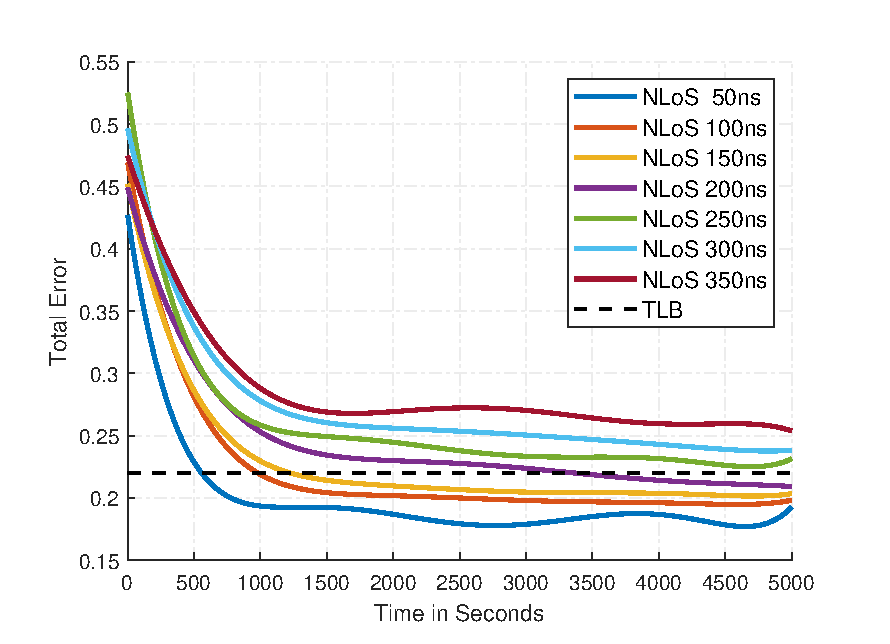
\includegraphics[width=0.5\textwidth]{7-T300-r200-V4-Exp-Changing-NLoS.eps}
\caption{\textcolor{red}{\textit{Training of NN-LVS. Training and test data is simulated with four BSs. $X_i$ has a fixed standard deviation of 300ns. $r$ is 200m. Standard deviation for NLoS is changing in training and test data set at the same time which is represented by different colour of curves in the figure.  TLB is the information theoretic Total Error lower bound. The Total Error for the NN-LVS increases with an increase in the NLoS bias.}}\label{New_1}}
\end{figure}

\textcolor{red}{\textit{Simulated ToA data is used in this work. The \emph{claimed} locations for genuine as well as malicious user-vehicles (in equal proportions) are generated randomly in the specified area and their respective ToAs is calculated at the four BSs. The malicious user-vehicle optimizes his true location at a distance $r$ from his claimed location. We use equation \eqref{optimal Px} to calculate $T_x^*$.}} The receivers in the BSs are under the influence of independent thermal noise $X_i$ and thus the ToA measurements they make have a certain degree of variation. We extract this variation (in nanoseconds) from a Gaussian random function that has a fixed standard deviation. \textcolor{red}{\textit{As described in equation \eqref{observ_H0} and \eqref{observ_H1}, NLoS bias, $\phi_i$, is added to the ToAs of the respective user-vehicles. To mimic reality, we extract the NLoS bias from an exponential distribution with a fixed standard deviation as highlighted in equation \eqref{exponential_bias}.}}

\textcolor{red}{\textit{We now take into account the TLB into our study in Fig.~\ref{New_1}. The TLB is calculated using equation \eqref{KL_te}. In the TLB calculation, $r$ is equal to 200m while the standard deviation for $X_i$ and NLoS bias is 300ns, and 900ns respectively. We assume this value of standard deviation for NLoS bias to closely relate to the global average for NLoS\footnote{\textcolor{red}{\textit{That is, we are assuming here that we have  \emph{a priori} knowledge on the channel conditions over some global average. We then use this TLB to provide a new stopping condition under a range of differing real-world test data. As we will see, there will be some test data where the TLB has no effect (usual stopping condition applies), and other test data where the stopping condition is reached well before the usual stopping condition. Even though the new training time is only about 1/5 of the usual training time, the  performance 'hit' is minimal.}}}. The calculated TLB with four BSs and the above settings is 0.22.}}

\textcolor{red}{\textit{For training the NN-LVS in Fig.~\ref{New_1}, we use a training data set which is simulated with an NLoS bias standard deviation of 50ns. Other simulation parameters are the same as those considered for the TLB calculations earlier. The training data has genuine and malicious user-vehicles in equal proportions. Prior to training the NN-LVS, the training data is randomized to closely mimic the reality. The NN-LVS is trained with the random user-vehicle data in each second and is further used to calculate a Total Error for the test data. Before re-training the NN-LVS and calculating a revised Total Error for the test data in each subsequent second, the previous training data is accumulated with the new random user-vehicle training data from that second. Total Error for the test data is plotted against time as shown in Fig.~\ref{New_1} (a polynomial fitting is applied). The figure also has Total Error curves for different values of NLoS bias standard deviation.}}

\textcolor{red}{\textit{In Fig.~\ref{New_3}, we carried out the same simulation as in Fig.~\ref{New_1} but revised the number of BSs to six. We did not change any of the other simulation parameters. One can see that the NN-LVS with six BSs performs better than the NN-LVS with four BSs. This highlights the fact that more number of BSs will result in better performance for the NN-LVS.}}

\begin{figure}[t!]
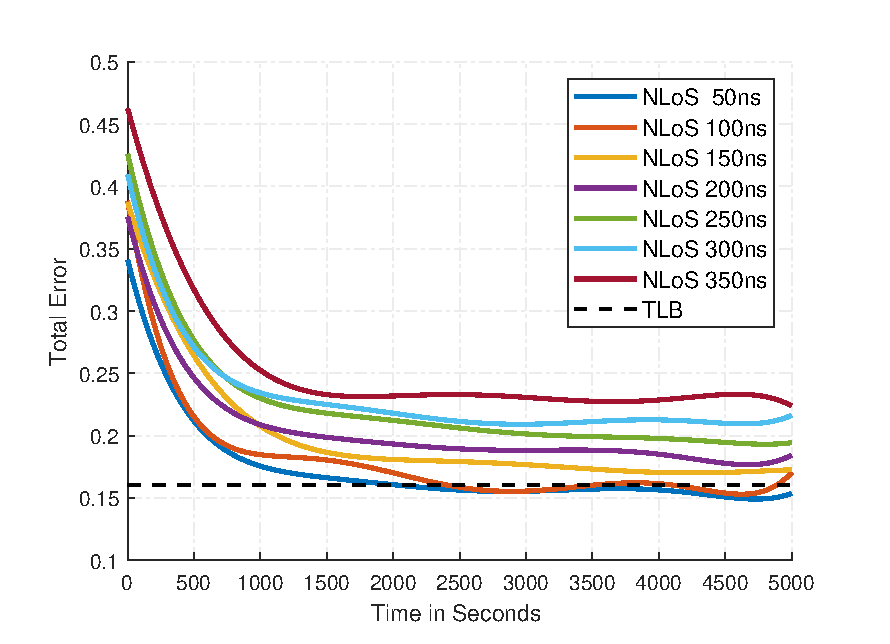
\includegraphics[width=0.50\textwidth]{7-T300-r200-V6-Exp-Changing-NLoS.eps}
\caption{\textcolor{red}{\textit{Training of the NN-LVS as in Fig.~\ref{New_1} except the number of BSs in this simulation has been modified to six.}}\label{New_3}}
\end{figure}

\textcolor{red}{\textit{In Fig.~\ref{New_6}, we study the impact of changing the BS's thermal noise, $X_i$, in terms of the Total Error for the NN-LVS. It is evident from this figure that NN-LVS shows an improved performance at lower values of $X_i$. The TLB in Fig.~\ref{New_6} has been calculated with $X_i$ = 300ns, NLoS bias equal to 900ns and $r$ = 200m. We see the case of $X_i$ = 300ns represents a scenario where the TLB would not be used as the stopping condition.}}

\begin{figure}[t!]
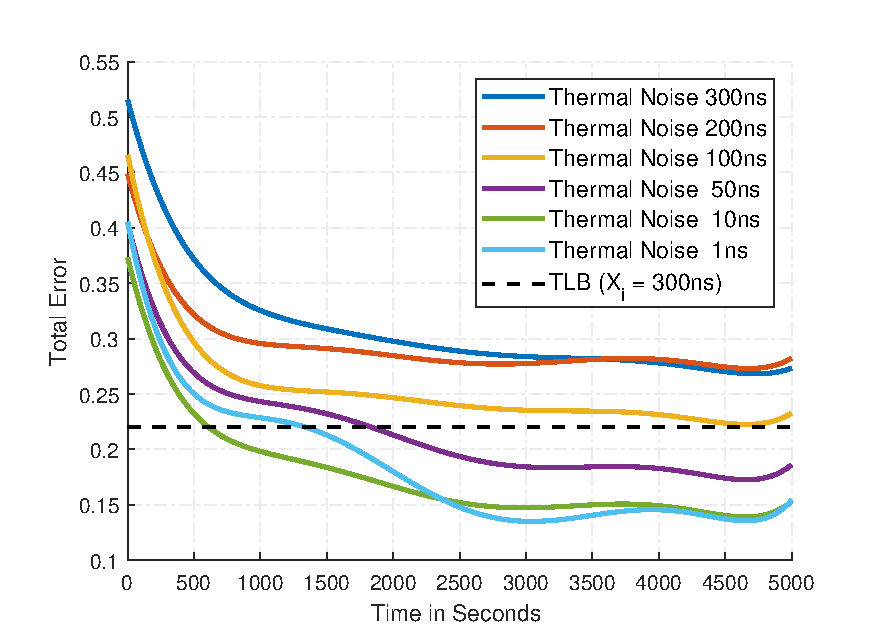
\includegraphics[width=0.50\textwidth]{7-N400-r200-V4-Exp-Changing-T.eps}
\caption{\textcolor{red}{\textit{NN-LVS performance with changing values of receivers thermal noise in the BSs. Other parameter settings in this simulation are: Standard deviation for NLoS is 400ns and the number of BSs are four. It can be seen that NN-LVS performs better with low receiver thermal noise.}}\label{New_6}}
\end{figure}

\textcolor{red}{\textit{We have carried out numerous numerical simulations of our trained NN-LVSs as applied to a wide range of data simulating real-world deployment.  The performance in term of the Total Error of the NN-LVSs is these tests show similar results to the flat parts of the curves shown in \Crefrange{New_1}{New_6}. That is, our NN-LVSs once trained perform as expected in our mimicked real-world deployments. In a nutshell, we see that when the NN-LVS training is stopped based on the TLB, we on average can cut the training time by a factor of $\frac{1}{5}$. That is, we can save training data costs and ensure quick deployment of the NN-LVS with minimal impact on the overall performance.}}

\section{Conclusion}
We have presented a new system for solving the important problem of location verification in the context of vehicular networks. Encompassing information theory and machine-learning concepts, the solutions we have provided will lead to enhanced and pragmatic location verification outcomes. Of particular importance is the fact that we have shown how a neural network based LVS is able to outperform a pure information-theoretic LVS when channel conditions are \emph{a priori} unknown and/or the malicious vehicle is at an unspecified distance from its claimed location.

We have also shown how optimal-information-theoretic concepts can be encapsulated with the machine learning framework so as to  allow for a very  useful trade-off in the training-time \emph{vs.} performance - thus making our solution even more practical in actual real-world deployment scenarios.

We hope our work will motivate others to undertake further research into the integration of machine-learning techniques and location verification. Verifying the location information utilized in vehicular networks is a problem of growing importance, and we believe the approach we have introduced here will eventually form the basis of all real-world solutions.

\section*{Acknowledgment}
The authors acknowledge support by the University of New South Wales, Australia, and Macquarie University, Australia. Ullah Ihsan acknowledges financial support from the Australian Government through its Research Training Program.

\begin{thebibliography}{1}

\bibitem{sheet2016location} D. Sheet, O. Kaiwartya, A. Abdullah, Y. Cao, A. Hassan, and S. Kumar, ``Location information verification using transferable belief model for geographic routing in vehicular ad hoc networks,'' \textit{IET Intelligent Transport Systems}, vol. 11, no. 2, pp. 53--60, Mar. 2017.

\bibitem{kasana2017location} R. Kasana,S. Kumar, O. Kaiwartya, W. Yan, Y. Cao and A. Abdullah, "Location Error Resilient Geographical Routing for Vehicular Ad-hoc Networks", IET Intelligent Transport Systems, Vol. 11, Issue 8, pp. 450 - 458, Oct. 2017.

\bibitem{yan2014optimal} S. Yan, R. Malaney, I. Nevat, and G. Peters, ``Optimal information-theoretic wireless location verification,'' \textit{IEEE Trans. Veh. Technol.}, vol. 63, no. 7, pp. 3410--3422, Jan. 2014.

\bibitem{yan2016location} S. Yan, I. Nevat, G. Peters, and R. Malaney, ``Location verification systems under spatially correlated shadowing,'' \textit{IEEE Trans. Wireless Commun.}, vol. 15, no.  6, pp. 4132--4144, Jun. 2016.

\bibitem{yan2016LOCATION} S. Yan, R. Malaney, I. Nevat, and G. Peters, ``Location verification systems for VANETs in Rician fading channels,'' \textit{IEEE Trans. Veh. Technol.}, vol. 65, no. 7, pp. 5652--5664, Jul. 2016.

\bibitem{monteiro2016information} M. Monteiro, J. Rebelatto, and R. Souza, ``Information-theoretic location verification system with directional antennas for vehicular networks,'' \textit{IEEE Trans. Intell. Transp. Syst.}, vol. 17, no. 1, pp. 93--103, Jan. 2016.

\bibitem{hartenstein2008tutorial} H. Hartenstein and L. P. Laberteaux, ``A tutorial survey on vehicular ad hoc networks,'' \textit{IEEE Commun. Mag.}, vol. 46, no. 6, pp. 164--171, Jun. 2008.

\bibitem{who} World Health Orginization, ``Number of road traffic deaths,'' Accessed on: July. 6, 2018, [Online]. Available: \underline{http://www.who.int/gho/road\_safety/mortality/traffic\_deaths\_number/en/}.

\bibitem{meneguetteintelligent} M. Rodolfo, D. Robson and L. Antonio, ``\textit{Intelligent Transport System in Smart Cities: Aspects and Challenges of Vehicular Networks and Cloud,}'', \nth{1} ed., Springer, 2018.

\bibitem{yan2013location} S. Yan, and R. Malaney, ``Location verification systems in emerging wireless networks,'' in \textit{ZTE Communications}, vol. 11, no. 3, pp. 03--10, Sep. 2013.

\bibitem{sastry2003secure} N. Sastry, U. Shankar, and D. Wagner, ``Secure verification of location claims,'' in \textit{Proc. ACM Workshop on Wireless Security}, Sep. 2003, pp. 1--10.

\bibitem{capkun2006secure} S. Capkun and J. P. Hubaux, ``Secure positioning in wireless networks,'' \textit{IEEE J. Sel. Areas Commun.}, vol. 24, no. 2, pp. 221--232, Feb. 2006.

\bibitem{leinmuller2006position} T. Leinm\"{u}ller, E. Schoch, and F. Kargl, ``Position verification approaches for vehicular ad hoc networks,'' \textit{IEEE Wireless Communications}, vol. 13, no. 5, pp. 16--21, Oct. 2006.

\bibitem{harsch2007secure}	C. Harsch, A. Festag, and P. Papadimitratos, ``Secure position-based routing for VANETs," in \textit{Proc. IEEE VTC}, Sep. 2007, pp. 26--30.

\bibitem{rasmussen2008secure}	S. Capkun, K. B. Rasmussen, M. Cagalj, and M. Srivastava, ``Secure location verification with hidden and mobile base stations,'' \textit{IEEE Trans. Mobile Comput.}, vol. 7, no. 4, pp. 470--483, Apr. 2008.

\bibitem{yan2008providing} G. Yan, S. Olariu, and M. C. Weigle, ``Providing VANET security through active position detection,'' \textit{Computer Communications}, vol. 31, no. 12, pp. 2883--2897, Jul. 2008.

\bibitem{zhang2012cooperative} P. Zhang, Z. Zhang, and A. Boukerche, ``Cooperative location verification for vehicular ad-hoc networks,'' in \textit{Proc. IEEE ICC}, Jun. 2012, pp. 37--41.

\bibitem{malandrino2013vip} F. Malandrino, C. Casetti, C. F. Chiasserini, M. Fiore, R. S. Yokoyama, and C. Borgiattino, ``A-VIP: Anonymous verification and inference of positions in vehicular networks,'' in \textit{Proc. IEEE INFOCOM}, Apr. 2013, pp. 105--109.

\bibitem{jaballah2013secure} W. Jaballah, M. Conti, M. Mosbah, and C. Palazzi, ``Secure verification of location claims on a vehicular safety application,'' in \textit{Proc. International Conference on Computer Communication and Networks}, Jul. 2013, pp. 1--7.

\bibitem{kim2017efficient} I. Kim, B. Kim, and J. Song, ``An efficient location verification scheme for static wireless sensor networks,'' \textit{Sensors}, vol. 17, no. 2, pp. 225--251, Jan. 2017.

\bibitem{caparra2017optimization} G. Caparra, M. Centenaro, N. Laurenti, and S. Tomasin, ``Optimization of anchor nodes' usage for location verification systems,'' in \textit{Proc. International Conference on Localization and GNSS (ICL-GNSS)}, Jun. 2017, pp. 1--6.

\bibitem{vaas2018get} C. Vaas, M. Juuti, N. Asokan, and I. Martinovic, ``Get in line: Ongoing co-presence verification of a vehicle formation based on driving trajectories,'' in \textit{Proc. IEEE European Symposium on Security and Privacy}, Apr. 2018.

\bibitem{fridman2017autonomous} L. Fridman, D. Brown, M. Glazer, W. Angell, and others, ``MIT autonomous vehicle technology study: Large-scale deep learning based analysis of driver behaviour and interaction with automation,'' arxiv 1711.06976, Nov. 2017.

\bibitem{Ausctw} S. Yan, R. Malaney, I. Nevat, and G. W. Peters, ``Timing information in wireless communications and optimal location verification frameworks,'' in \textit{Proc Australian Communications Theory Workshop (AusCTW)}, Feb. 2014, pp. 144--149.

\bibitem{Ihsan_ICC} U. Ihsan, Z. Wang, R. Malaney, A. Dempster, and S. Yan, ``Artificial intelligence and location verification in vehicular networks'', submitted to \textit{IEEE ICC}, 2018.

%\bibitem{yan2012information} S. Yan, R. Malaney, I. Nevat, and G. Peters, ``An information theoretic location verification system for wireless networks,'' in \textit{Proc. IEEE GlobeCOM}, Dec. 2012, pp. 5415--5420.

\bibitem{neyman1933problem} J. Neyman and E. Pearson, ``On the problem of the most efficient tests of statistical hypotheses,'' \textit{Phil. Trans. R. Soc. A}, vol. 231, pp. 289--337,  1933.

\bibitem{gradshteuin2007table} Gradshteyn, I. S., and Ryzhik, I. M, ``\textit{Table of Integrals, Series and Products,}'' \nth{7} ed., Academic, San Diego, CA, 2007.

\bibitem{lehmann2005testing} E. Lehmann and J. Romano, ``\textit{Testing Statistical Hypotheses,}'' 3rd ed. New York: Springer Science \& Business Media, 2006.

\bibitem{yan2018delay} S. Yan, B. He, X. Zhou, Y. Cong, and A. L. Swindlehurst, ``Delay-intolerant covert communications with either fixed or random transmit power,'' \emph{IEEE Trans. Inf. Forensics Security}, Early Access, Jun. 2018.

\end{thebibliography}

\end{document}
